\cleardoublepage
\chapter{Results}
\label{chap:results}

This chapter presents the empirical results for Lazy VFDT and Dynamic Weighted Majority (DWM) across the synthetic and real-world datasets described earlier. Metrics are aggregated over five seeds unless noted otherwise; detailed numbers appear in \texttt{docs/results\_summary.md} and Figures~\ref{fig:accuracy}, \ref{fig:training-time}, and \ref{fig:avg-latency}.

\section{Rotating Hyperplane (Drift Rate 0.05)}
Lazy VFDT achieved a mean accuracy of 75.8\% (\(\pm 12.6\) points) compared to 69.3\% (\(\pm 10.4\)) for DWM. Training time was 0.07~s for Lazy VFDT versus 7.22~s for DWM, with average prediction latency of 0.01~ms vs. 0.08~ms. The tree remained compact (mean 87 nodes) while DWM maintained a single expert due to aggressive pruning.

\section{Electricity}
On the ELEC2 dataset, Lazy VFDT outperformed DWM by approximately 8 percentage points (64.7\% vs. 56.5\% accuracy) while training roughly 90 times faster (0.31~s vs. 28.1~s). Average latency stayed below 0.01~ms for Lazy VFDT, whereas DWM incurred 0.09~ms due to ensemble voting. Model sizes remained modest (52 nodes for Lazy VFDT, 2 experts for DWM).

\section{Gas Sensor Array Drift}
With per-batch scaling and deeper trees, Lazy VFDT reached 22.1\% accuracy (\(\pm 7.1\)) versus 14.3\% (\(\pm 3.7\)) for DWM. Although absolute accuracy is low due to the six-class drift challenge, Lazy VFDT retained the latency advantage (0.01~ms vs. 0.08~ms) and trained in under a second (0.97~s vs. 29.7~s). Tree size grew substantially (mean 481 nodes) reflecting the complexity of the task.

\section{Airlines}
For the Airlines stream, DWM delivered slightly higher accuracy (52.7\%) than Lazy VFDT (49.6\%) but at a significant computational cost: training required 1{,}150~s per run (with a large sliding window), while Lazy VFDT trained in 6.2~s. Latency also favoured Lazy VFDT (0.02~ms vs. 0.12~ms). This highlights the trade-off between squeezing out a few extra accuracy points and maintaining practical efficiency.

\section{Figures}
\begin{figure}[!h]
    \centering
    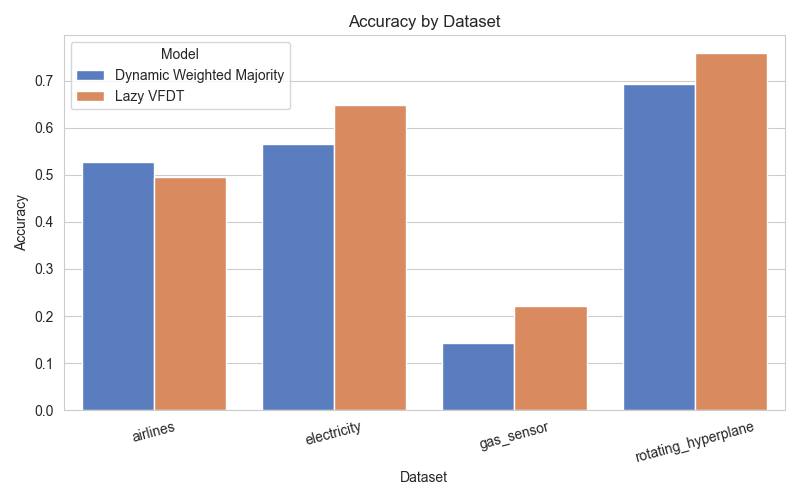
\includegraphics[width=0.8\linewidth]{tex/img/accuracy.png}
    \caption{Accuracy comparison across datasets.}
    \label{fig:accuracy}
\end{figure}

\begin{figure}[!h]
    \centering
    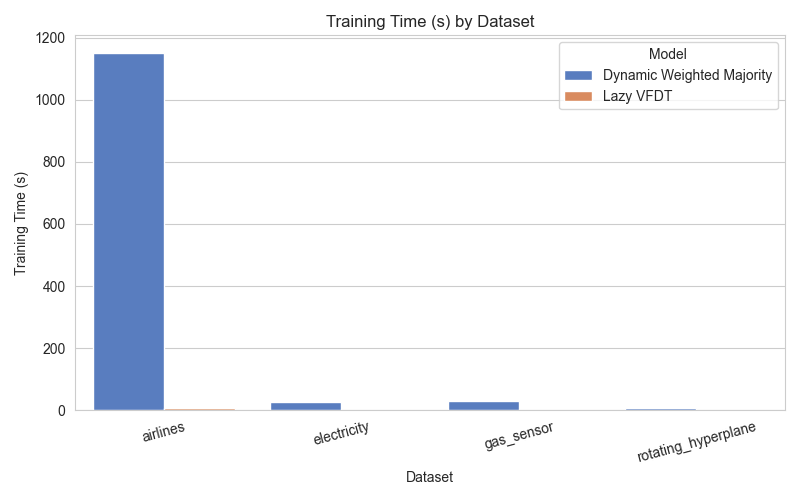
\includegraphics[width=0.8\linewidth]{tex/img/training_time.png}
    \caption{Training time comparison (log-scale recommended when presenting).}
    \label{fig:training-time}
\end{figure}

\begin{figure}[!h]
    \centering
    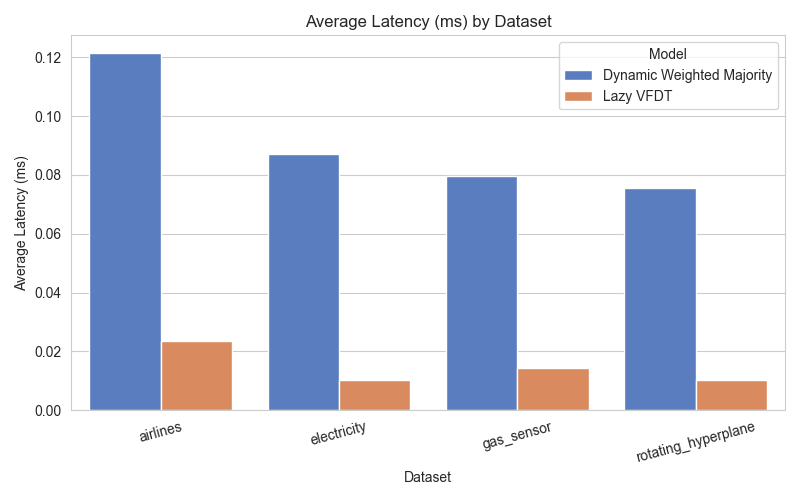
\includegraphics[width=0.8\linewidth]{tex/img/avg_latency.png}
    \caption{Average prediction latency comparison.}
    \label{fig:avg-latency}
\end{figure}

The figures emphasise Lazy VFDT’s consistent efficiency gains, even when DWM occasionally edges accuracy (e.g., Airlines).

